\chapter{The Epsilon Transformation Language (ETL)}
\label{sec:ETL}

The aim of ETL \cite{ETL} is to contribute model-to-model transformation capabilities to Epsilon. More specifically, ETL can be used to transform an arbitrary number of input models into an arbitrary number of output models of different modelling languages and technologies at a high level of abstraction. 

\section{Style}

Three styles are generally recognized in model transformation languages: declarative, imperative and hybrid, each one demonstrating particular advantages and shortcomings. Declarative transformation languages are generally limited to scenarios where the source and target metamodels are similar to each other in terms of structure and thus, the transformation is a matter of a simple mapping. However they fail to address cases where significant processing and complex mappings are involved. On the other hand, purely imperative transformation languages are capable of addressing a wider range of transformation scenarios. Nevertheless, they operate at a low level of abstraction which means that users need to manually address issues such as tracing and resolving target elements from their source counterparts and orchestrating the transformation execution. To address those shortcomings, hybrid languages (such as ATL \cite{ATL} and QVT \cite{QVT}) provide both a declarative rule-based execution scheme as well as imperative features for handling complex transformation scenarios. 

Under this rationale, ETL has been designed as a hybrid language that implements a task-specific rule definition and execution scheme but also inherits the imperative features of EOL to handle complex transformations where this is deemed necessary.

\section{Source and Target Models}

The majority of model-to-model transformation languages assume that only two models participate in each transformation: the source model and the target model. Nevertheless, it is often essential to be able to access/update additional models during a transformation (such as trace or configuration models). Building on the facilities provided by EMC and EOL, ETL enables specification of transformations that can transform an arbitrary number of source models into an arbitrary number of target models.

Another common assumption is that the contents of the target models are insignificant and thus a transformation can safely overwrite its contents. As discussed in the sequel, ETL - like all Epsilon languages - enables the user to specify, for each involved model, whether its contents need to be preserved or not.

\section{Abstract Syntax}

As illustrated in Figure \ref{fig:EtlAbstractSyntax}, ETL transformations are organized in modules (\emph{EtlModule}). A module can contain a number of transformation rules (\emph{TransformationRule}). Each rule has a unique name (in the context of the module) and also specifies one \emph{source} and many \emph{target} parameters. A transformation rule can also \emph{extend} a number of other transformation rules and be declared as \emph{abstract}, \emph{primary} and/or \emph{lazy}\footnote{The concept of lazy rules was first introduced in ATL}. To limit its applicability to a subset of elements that conform to the type of the \emph{source} parameter, a rule can optionally define a guard which is either an EOL expression or a block of EOL statements. Finally, each rule defines a block of EOL statements (\emph{body}) where the logic for populating the property values of the target model elements is specified.

Besides transformation rules, an ETL module can also optionally contain a number of \emph{pre} and \emph{post} named blocks of EOL statements which, as discussed later, are executed before and after the transformation rules respectively. These should not be confused with the pre-/post-condition annotations available for EOL user-defined operations (Section~\ref{sec:prep-cond-user}).

\begin{landscape}
\begin{figure}
	\centering
		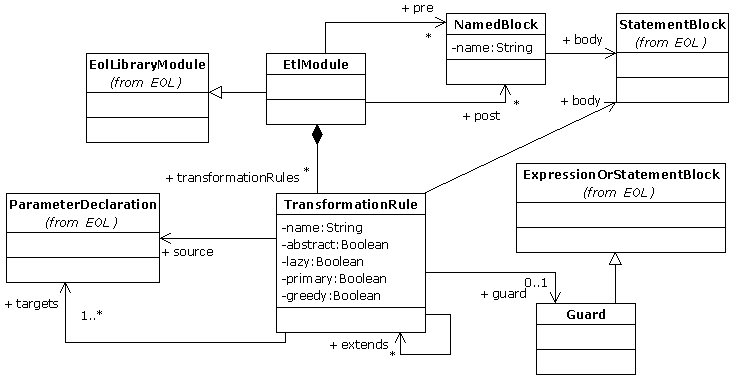
\includegraphics{images/EtlAbstractSyntax.png}
	\caption{ETL Abstract Syntax}
	\label{fig:EtlAbstractSyntax}
\end{figure}
\end{landscape}

\section{Concrete Syntax}

The concrete syntax of a transformation rule is displayed in Listing \ref{lst:TransformationRuleConcreteSyntax}. The optional \emph{abstract}, \emph{lazy} and \emph{primary} attributes of the rule are specified using respective annotations. The name of the rule follows the \emph{rule} keyword and the \emph{source} and \emph{target} parameters are defined after the \emph{transform} and \emph{to} keywords. Also, the rule can define an optional comma-separated list of rules it extends after the \emph{extends} keyword. Inside the curly braces (\{\}), the rule can optionally specify its \emph{guard} either as an EOL expression following a colon (:) (for simple guards) or as a block of statements in curly braces (for more complex guards). Finally, the \emph{body} of the rule is specified as a sequence of EOL statements.

\begin{lstlisting}[caption=Concrete Syntax of a TransformationRule, label=lst:TransformationRuleConcreteSyntax, language=ETL, escapechar=!]
(@abstract)?
(@lazy)?
(@primary)?
rule !\textit{<name>}!
	transform !\textit{<sourceParameterName>}\textbf{:}\textit{<sourceParameterType>}!
	to !\textit{<rightParameterName>}\textbf{:}\textit{<rightParameterType>}!
	    (!\textbf{,} \textit{<rightParameterName>}\textbf{:}\textit{<rightParameterType>}!)*
	(extends !\textit{<ruleName>}!(!\textbf{,} \textit{<ruleName>}!)*)? {
	
	(guard (!\textbf{:}\textit{expression}!)|(!\textbf{\{}\textit{statementBlock}\textbf{\}}!))?
	
	!\textit{statement}!+
}
\end{lstlisting}

\emph{Pre} and \emph{post} blocks have a simple syntax that, as presented in Listing \ref{lst:EtlPrePostConcreteSyntax}, consists of the identifier (\emph{pre} or \emph{post}), an optional name and the set of statements to be executed enclosed in curly braces.

\begin{lstlisting}[caption=Concrete Syntax of Pre and Post blocks, label=lst:EtlPrePostConcreteSyntax, language=ETL]
(pre|post) <name> {
	statement+
}
\end{lstlisting}

\section{Execution Semantics}
\label{sec:ETL.ExecutionSemantics}

\subsection{Rule and Block Overriding}
Similarly to ECL, an ETL module can import a number of other ETL modules. In this case, the importing ETL module inherits all the rules and pre/post blocks specified in the modules it imports (recursively). If the module specifies a rule or a pre/post block with the same name, the local rule/block overrides the imported one respectively.

\subsection{Rule Execution Scheduling}

When an ETL module is executed, the \emph{pre} blocks of the module are executed first in the order in which they have been specified. 

Following that, each \emph{non-abstract} and \emph{non-lazy} rule is executed for all the elements on which it is applicable. To be applicable on a particular element, the element must have a type-of relationship with the type defined in the rule's \emph{sourceParameter} (or a kind-of relationship if the rule is annotated as \emph{@greedy}) and must also satisfy the \emph{guard} of the rule (and all the rules it extends). When a rule is executed on an applicable element, the target elements are initially created by instantiating the \emph{targetParameters} of the rules, and then their contents are populated using the EOL statements of the \emph{body} of the rule.

Finally, when all rules have been executed, the \emph{post} blocks of the module are executed in the order in which they have been declared.

\subsection{Source Elements Resolution}

Resolving target elements that have (or can be) transformed from source elements by other rules is a frequent task in the body of a transformation rule. To automate this task and reduce coupling between rules, ETL contributes the \emph{equivalents()} and \emph{equivalent()} built-in operations that automatically resolve source elements to their transformed counterparts in the target models. 

When the \emph{equivalents()} operation is applied on a single source element (as opposed to a collection of them), it inspects the established transformation trace (displayed in Figure \ref{fig:EtlRuntime}) and invokes the applicable rules (if necessary) to calculate the counterparts of the element in the target model. When applied to a collection it returns a \emph{Bag} containing \emph{Bags} that in turn contain the counterparts of the source elements contained in the collection. The \emph{equivalents()} operation can be also invoked with an arbitrary number of rule names as parameters to invoke and return only the equivalents created by specific rules. Unlike the main execution scheduling scheme discussed above, the \emph{equivalents()} operation invokes both \emph{lazy} and \emph{non-lazy} rules. It is worth noting that \emph{lazy} rules are computationally expensive and should be used with caution as they can significantly degrade the performance of the overall transformation.

With regard to the ordering of the results of the \emph{equivalents()} operations, the returned elements appear in the respective order of the rules that have created them. An exception to this occurs when one of the rules is declared as \emph{primary}, in which case its results precede the results of all other rules.

\begin{landscape}
\begin{figure}
	\centering
		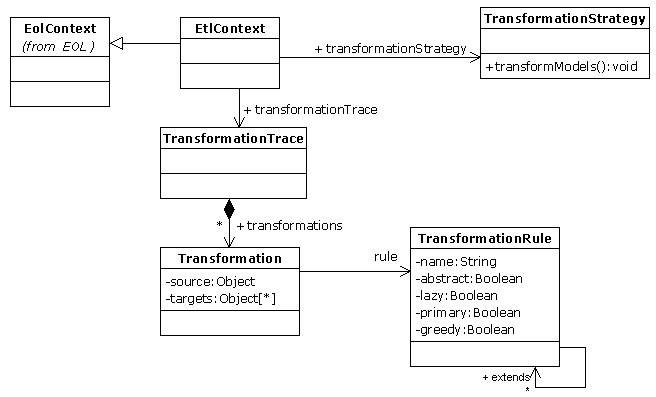
\includegraphics{images/EtlRuntime.png}
	\caption{ETL Runtime}
	\label{fig:EtlRuntime}
\end{figure}
\end{landscape}


ETL also provides the convenience \emph{equivalent()} operation which, when applied to a single element, returns only the first element of the respective result that would have been returned by the \emph{equivalents()} operation discussed above. Also, when applied to a collection the \emph{equivalent()} operation returns a flattened collection (as opposed to the result of \emph{equivalents()} which is a \emph{Bag} of \emph{Bags} in this case). As with the \emph{equivalents()} operation, the \emph{equivalent()} operation can also be invoked with or without parameters.

The semantics of the \emph{equivalent()} operation are further illustrated through a simple example. In this example, we need to transform a model that conforms to the Tree metamodel displayed in Figure \ref{fig:Tree} into a model that conforms to the Graph metamodel of Figure \ref{fig:Graph}. More specifically, we need to transform each \emph{Tree} element to a \emph{Node}, and an \emph{Edge} that connects it with the \emph{Node} that is equivalent to the tree's \emph{parent}. This is achieved using the rule of Listing \ref{lst:SimpleETLTransformationRule}. 

\begin{lstlisting}[float=h, caption=Exemplar ETL Rule demonstrating the \emph{equivalent()} operation, label=lst:SimpleETLTransformationRule, language=ETL, escapechar=\#]
rule Tree2Node#\label{lst:etl-simple-def-start}#
	transform t : Tree!Tree
	to n : Graph!Node {#\label{lst:etl-simple-def-end}#
	
	n.label = t.label;#\label{lst:etl-simple-label}#
	
	if (t.parent.isDefined()) {#\label{lst:etl-simple-sourceisdef}#
		var edge = new Graph!Edge;#\label{lst:etl-simple-newedge}#
		edge.source = n;#\label{lst:etl-simple-source}#
		edge.target = t.parent.equivalent();#\label{lst:etl-simple-equiv}#
	}
}
\end{lstlisting}


In lines \ref{lst:etl-simple-def-start}--\ref{lst:etl-simple-def-end}, the \emph{Tree2Node} rule specifies that it can transform elements of the \emph{Tree} type in the \emph{Tree} model into elements of the \emph{Node} type in the \emph{Graph} model. In line~\ref{lst:etl-simple-label} it specifies that the name of the created Node should be the same as the name of the source Tree. If the parent of the source \emph{Tree} is defined (line~\ref{lst:etl-simple-sourceisdef}), the rule creates a new \emph{Edge} (line~\ref{lst:etl-simple-newedge}) and sets its \emph{source} property to the created \emph{Node} (line~\ref{lst:etl-simple-source}) and its \emph{target} property to the \emph{equivalent} \emph{Node} of the source \emph{Tree}'s \emph{parent} (line~\ref{lst:etl-simple-equiv}).

\begin{figure}
	\centering
		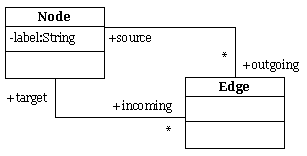
\includegraphics{images/Graph.png}
	\caption{A Simple Graph Metamodel}
	\label{fig:Graph}
\end{figure}


\subsection{Overriding the semantics of the EOL SpecialAssignmentOperator}
\label{sec:Design.ETL.SpecialAssignmentOperator}

As discussed above, resolving the equivalent(s) or source model elements in the target model is a recurring task in model transformation. Furthermore, in most cases resolving the equivalent of a model element is immediately followed by assigning/adding the obtained target model elements to the value(s) of a property of another target model element. For example, in line 10 of Listing \ref{lst:SimpleETLTransformationRule} the \emph{equivalent} obtained is immediately assigned to the \emph{target} property of the generated \emph{Edge}. To make transformation specifications more readable, ETL overrides the semantics of the \emph{SpecialAssignmentStatement} (\emph{::=} in terms of concrete syntax), described in Section \ref{sec:Design.EOL.SpecialAssignmentStatement} to set its left-hand side, not to the element its right-hand side evaluates to, but to its \emph{equivalent} as calculated using the \emph{equivalent()} operation discussed above. Using this feature, line 10 of the \emph{Tree2Node} rule can be rewritten as shown in Listing \ref{lst:SpecialAssignmentETLTransformationRule}

\begin{lstlisting}[caption=Rewritten Line 10 of the \emph{Tree2Node} Rule Demonstrated in Listing \ref{lst:SimpleETLTransformationRule}, label=lst:SpecialAssignmentETLTransformationRule, language=ETL]
edge.target ::= t.parent;
\end{lstlisting}


\section{Interactive Transformations}
\label{sec:InteractiveModelTransformation}

Using the user interaction facilities of EOL discussed in Section \ref{sec:Design.EOL.UserInput}, an ETL transformation can become interactive by prompting the user for input during its execution. For example in Listing \ref{lst:InteractiveETLTransformationRule}, we modify the \emph{Tree2Node} rule originally presented in Listing \ref{lst:SimpleETLTransformationRule} by adding a \emph{guard} part that uses the user-input facilities of EOL (more specifically the \emph{UserInput.confirm(String,Boolean)} operation) to enable the user select manually at runtime which of the Tree elements need to be transformed to respective Node elements in the target model and which not. 

\begin{lstlisting}[caption=Exemplar Interactive ETL Transformation, label=lst:InteractiveETLTransformationRule, language=ETL]
rule Tree2Node
	transform t : Tree!Tree
	to n : Graph!Node {
	
	guard : UserInput.confirm
		("Transform tree " + t.label + "?", true)
	
	n.label = t.label;
	var target : Graph!Node ::= t.parent;
	if (target.isDefined()) {
		var edge = new Graph!Edge;
		edge.source = n;
		edge.target = target;
	}
}
\end{lstlisting}

\section{Summary}

This section has provided a detailed discussion on the Epsilon Transformation Language (ETL). ETL is capable of transforming an arbitrary number of source models into an arbitrary number of target models. ETL adopts a hybrid style and features declarative rule specification using advanced concepts such as \emph{guards}, \emph{abstract}, \emph{lazy} and \emph{primary} rules, and automatic resolution of target elements from their source counterparts. Also, as ETL is based on EOL reuses its imperative features to enable users to specify particularly complex, and even interactive, transformations.